\label{introTA}
% ===================================================
\section{Problem Statement}
% ===================================================
In this Part, we consider a two-agent pursuit-evasion problem that involves  a Target (aircraft) in opposition to an Attacker (missile). The Target tries to evade the Attacker and avoid being captured by him. We will try to find a simple technique for target evasion, so we should have a look at evasion techniques.
%The missile is on the ground, its position is (0,0). The plane is flaying is the air, its position is (10000,40000).

\section{Evasion techniques}

Each missile type has its own fundamental weaknesses and though some of these weaknesses or limitations may be kept secret by the missile’s manufacturer, many of them can be easily inferred by the manufacturer's opponents through observation. Propulsion is one of the most prominent limitations of any missile. Most contemporary missiles employ rocket propulsion which enjoys the two advantages of a high thrust/weight ratio and a small size. The typical thrust profile of such a propellant rocket is that of an initial high impulse burn to accelerate up to cruise speed, which is followed by a slower sustainer burn. Once the propellant is burned out, the rocket will continue due to inertia until drag takes its toll. The maneuvering ability of such a missile depends critically on its speed and therefore the amount of wing and body lift it can generate. Immediately after launch the missile has poor maneuverability due to its low speed, but this improves as its cruise speed is reached. Maneuverability will peak at the instant when the sustainer is about to burn out as the weapon has its lowest mass and a high energy state while still possessing powerplant thrust. After sustainer burnout, the missile will bleed off its energy which reduces its ability to follow through maneuvers. Ideally, a missile airframe will employ a combination of wing and body lift to provide maximum turn rate with minimum energy bleed throughout all phases of its flight while maximizing range.\\

The aircraft must exploit every known weakness of the missile's system to defeat the missile. Missiles are a visible threat which act on a timescale that allows some tangible response. An aircraft maximizes its chances of survival by maintaining a high energy state, and by possessing a system of early and accurate warning. Figure \ref{Evasion Taxonomy} displays tree-like taxonomy of the techniques that can be used by an aircraft to avoid being hit by an attacking missile. The figure shows that there are two main classes of such techniques. The first class is that of kinematics-based tactics (maneuvers) and is, in fact, the genuine class of evasion techniques studied in aeronautical engineering and is the class of interest in this thesis. The second class of evasion techniques are not based on kinematics but are of proven practical utility.  The advent of Fourth Generation Air-Air Missiles (AAMs) and 'double digit' Surface-Air missiles (SAMs) has somewhat decreased what could be achieved by using maneuver techniques. Nevertheless, these techniques remain effective against many conventional and legacy weapons, provided the aircraft has the required performance capabilities. Kinematics-based techniques are still of paramount importance form both the theoretical and practical points of view.



\begin{figure}[H]
	\centering
	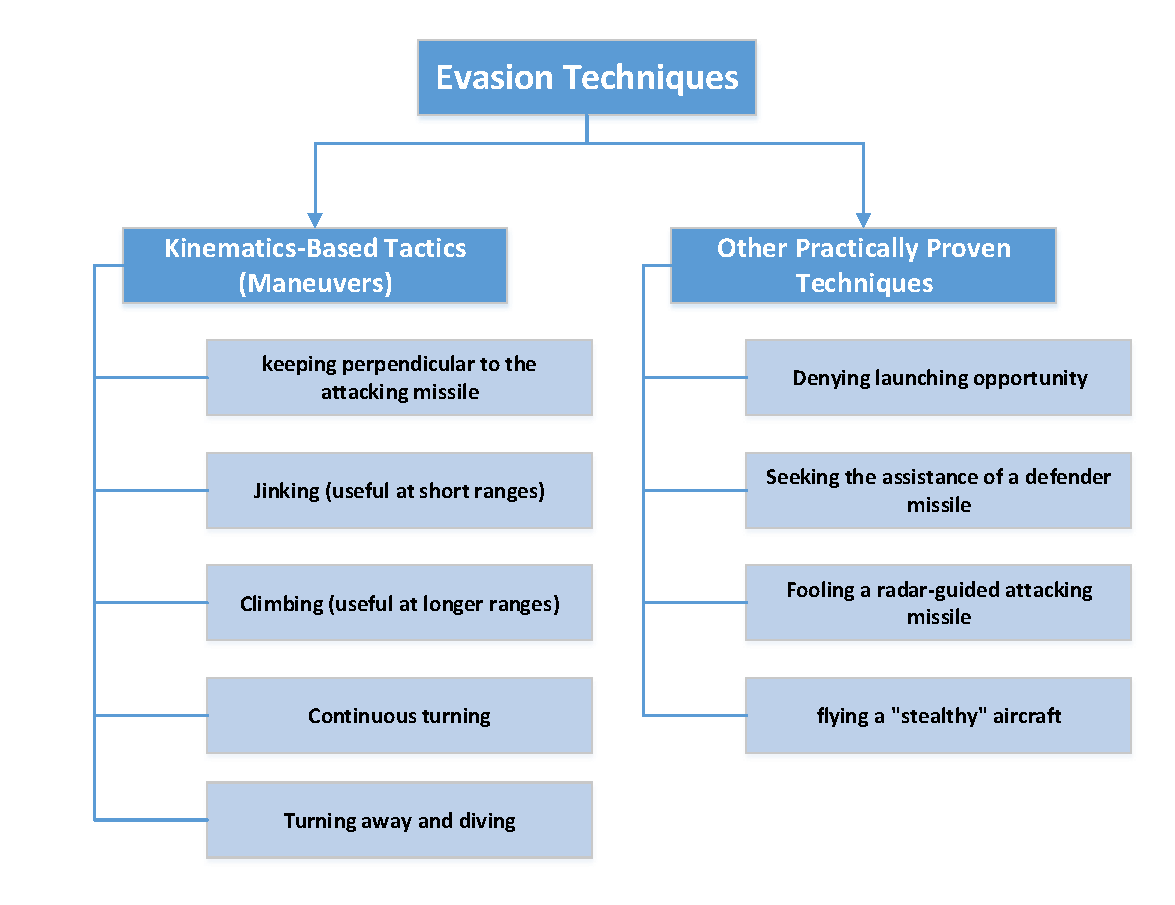
\includegraphics[scale = 0.9]{fig/Evasion.pdf}
	\caption{Taxonomy of evasion techniques}
	\label{Evasion Taxonomy}
\end{figure}

Before explaining the taxonomy given in Figure \ref{Evasion Taxonomy}, we list a few useful observations, namely  
\begin{itemize}
	\item The missile is typically faster than the aircraft (otherwise, the aircraft can evade the missile by simply running away from it without having to maneuver).
	\item The missile cannot turn tighter than the aircraft, so it takes a longer path.
	\item The control mechanism of the missile is much simpler and is of less capability than that of the aircraft. In order to pull as tight turn as the aircraft, it must exercise an acceleration that is far beyond its capability.
	\item The missile always attempts to trace the target and not to lead it. Thus, if the target changes heading, it will be necessary for the Missile to change heading similarly, but this is too difficult for it to achieve.
	\item  The main problem for an aircraft when evading a missile is how to compensate for the missile's speed superiority. This makes timing a somewhat critical issue for the aircraft.
\end{itemize}
\textbf{The most important kinematics-based evasion techniques are :}
\begin{enumerate}
	\item \textbf{keeping perpendicular to the attacking missile:}\\
	Perpendicularity evading is the maneuver technique used when the missile is fired head-on at a beyond visual range (BVR). The target turns hard to either left or right so as to fly at roughly a 90 degrees angle to the attacking missile. This perpendicular orientation or beam aspect (3 o'clock position or 9 o'clock position) should allow visual acquisition and tracking of the incoming missile, particularly if it is originally fired from 6 o'clock position. 
	Perpendicularity evading forces the missile to bleed off its energy and to possibly lead the target. Once the target aircraft makes a hard turn to reverse its direction, the missile with its far larger turn circle will be unable to compensate. The aircraft might have to constantly maneuver to keep perfectly perpendicular to the missile to keep it from locking on to it. Figure \ref{1st evasion tech} illustrates the perpendicularity evading maneuver technique.
	
					\begin{figure}[H]
					 	\centering
					 	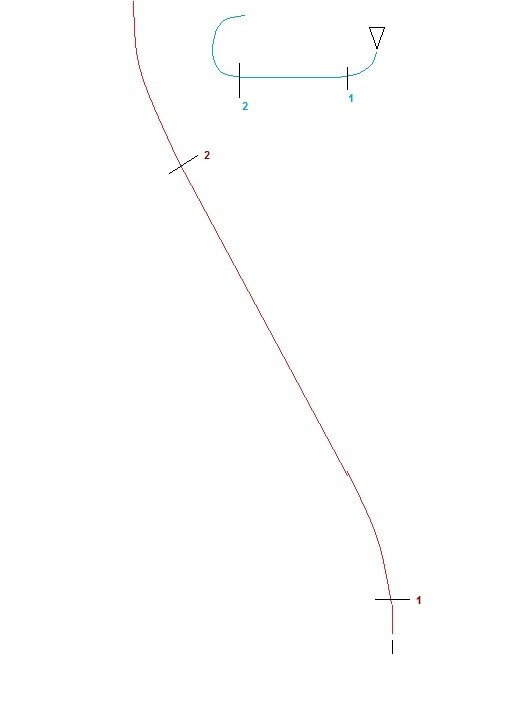
\includegraphics[scale = 0.45]{fig/evasiontech1.jpg}
					 	\caption{Illustration of the perpendicularity evading maneuver technique}
					 	\label{1st evasion tech}
					 \end{figure}
	\item \textbf{ Jinking (useful at short ranges):}\\
	The word "jinking" means literally "to suddenly change direction" and essentially belongs to the specialized jargon of aeronautical engineering. In the jinking maneuver, the aircraft must be positioned so that it is at an acute angle (30-60 degrees are optimum) relative to the missile’s flight path. Once the missile gets closer, the aircraft will make a hard turn in the opposite direction. As there is a time lag between the aircraft changing its direction and the missile following it (for several reasons, most important of which is the missile’s inertia), this will cause the missile to head in the wrong direction until it manages to correct, and also to bleed off its limited energy. Usually the missile will fly past the aircraft and miss. Figure \ref{jinking} illustrates the jinking evading maneuver technique.
					\begin{figure}[H]
						 \centering
						 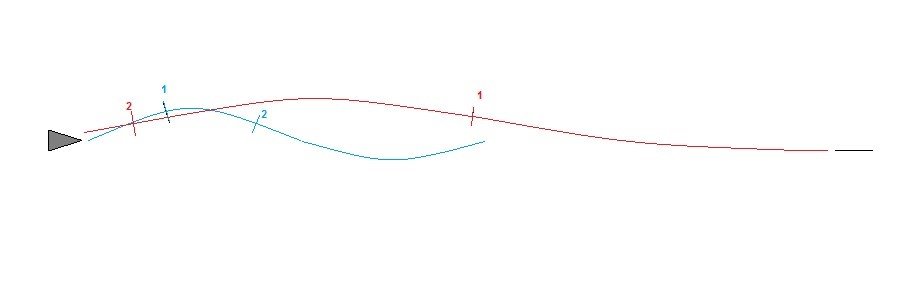
\includegraphics[scale = 0.7]{fig/evasiontech2.jpg}
						 \caption{Illustration of the jinking maneuver technique}
						 \label{jinking}
					\end{figure}
	\item  \textbf{Climbing  (useful at longer ranges):}\\
	Since at a long range the missile will have burned out its engine, it will rely on inertia to keep flying, and climbing will mean that it will bleed off energy rapidly. Once the missile reaches a close range (maybe around 1,500 meters), the aircraft should dive for the ground, then pull up. This will allow the aircraft to gain kinematic energy and use it to evade the missile. Figure \ref{climb} illustrates the climbing evading maneuver technique.
			\begin{figure}[H]
				\centering
				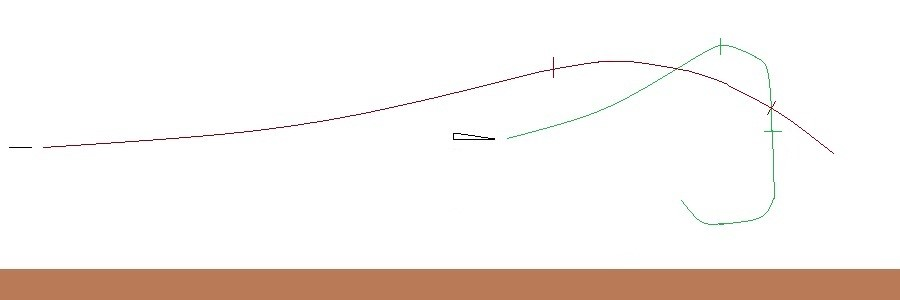
\includegraphics[scale = 0.7]{fig/evasiontech3.jpg}
				\caption{Illustration of the climbing maneuver technique}
				\label{climb}
			\end{figure}
	\item \textbf{Continuous turning:}\\
	The aircraft places the missile at a 3 o’clock or a 9 o’clock position. It then maintains a sufficient turn to keep the missile turning all the time. This tactic forces the missile to execute a continuous turn, bleeding its energy the entire time, making it easier for the aircraft to outturn the missile once it comes close. Figure \ref{Continuous turning} illustrates the continuous turning maneuver technique.
			\begin{figure}[H]
			\centering
			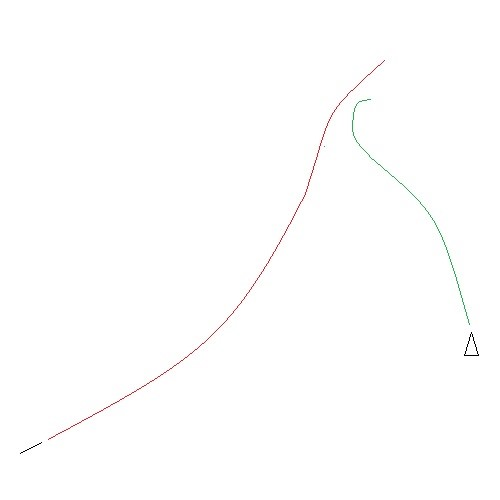
\includegraphics[scale = 0.7]{fig/evasiontech4.jpg}
			\caption{Illustration of the continuous turning maneuver technique}
			\label{Continuous turning}
			\end{figure}
		
	\item \textbf{Turning away and diving :}\\	
	The aircraft turns away from the attacking missile and dives for the ground, gaining speed and putting as much distance as possible between itself and the missile. This tactic is not useful on its own at shorter ranges, and the pilot must evade the missile physically by pulling the aircraft into the turn and forcing the missile to overshoot once the missile comes sufficiently close. This "Going to ground" tactic also confuses the missile's guidance via "back scatter" from objects on the ground
\end{enumerate}


To make this thesis self-contained, we now add a brief description of other practical evasion techniques that are not of kinematic origin, and are therefore outside the main scope of this thesis: 

\begin{enumerate}
	\item \textbf{Denying launching opportunity:}\\
	The famous proverb "\textit{prevention is better than cure}" indicates that it is better to stop something undesirable from happening than it is to deal with it after it has already happened. Therefore, the best tactic for the aircraft when dealing with Surface-Air missile (SAM) sites is to prevent the launching of a missile by remaining safely outside of the known envelope or launching cone of the missile. This tactic is called the maneuver of denying the missile-launching site an opportunity to shoot. In fact, flying over SAM-infested hostile territory is asking to get hit, and should be avoided by all means. Of course, the tactic of denying launching opportunity is not an evasion one per se, albeit it is a very prudent one, indeed. In line with this tactic is the fact that the first mission objective in any offensive air operation is to destroy every hostile radar and SAM installation.
	
	\item \textbf{Seeking the assistance of a defender missile:}\\
	The aircraft (or some of its air or surface allies) might launch a defender missile to intercept and stop the attacking missile, hopefully before this attacker reaches it. This kind of active evasion changes our current TA problem to the more sophisticated TAD problem, to be discussed in the second part of this thesis.
	
	\item \textbf{Fooling a radar-guided attacking missile:}\\
	Physically avoiding the enemy missile is not the only option for a targeted aircraft. If the missile is radar-guided, it can be misguided, decoyed, fooled, or deceived by the aircraft via electronic signal jamming or by dispensing or deploying a bundle of flares and chaff (tiny metal pieces) followed by changing course. The missile is caused to lose lock on the target and have either a miss or a premature detonation (When missiles lose the lock they either self-destruct or continue flying in a straight course). The aircraft might receive assistance from nearby friendly planes for jamming enemy radar on a broad range of frequencies (typically hostile ones).
	
	\item \textbf{Flying a "stealthy" aircraft:}\\
	Modern stealthy aircrafts have extremely small radar cross-sections, are impossibly quiet, are hard to see in the day or night, and have a heat signature not that much warmer than the ground they fly over. No one can target what radars, heat sensors, and human eyes and ears cannot detect. Drones are particularly effective with stealth, as the lack of need to support a pilot can grant them a cross-section smaller than a bird on radar. A very hot area of research in electromagnetics nowadays is to develop meta-materials that are essentially invisible over a broad band of frequencies. 
	
\end{enumerate}


%Why use polynomials?
Now we want to search for a path that the Target can move on it to escape from the Attacker. All the evasion techniques depend on the time of the turn that the Target makes when it detects the Attacker (Missile) and the objective is to maximize the Missile acceleration till the Missile power bleed. 
We will  choose the escaping trajectory as a polynomial with unknown coefficients, then try to find these coefficients which make the Missile exert a maximum acceleration to bleed its power as fast as we can before it reaches the Target.  
% ===================================================
\section{Assumptions, Notation, and Nomenclature}
% ===================================================
\subsection*{Assumptions}

\begin{enumerate}
	\item Both the Attacker and Target travel at constant speeds.
	\item The Attacker's speed is larger than that of the Target. Otherwise, the Target will be unconditionally or trivially capable of escaping. 
	\item Gravitational and drag effects are neglected for simplicity.
	\item The maximum g-force a typical person can handle is 5G
	\item The maximum g-force a pilot fighter (with safety equipments) could resist is 10G.
	\item The maximum g-force for a sprint missile is 100G.
	\item The range for Tactical missile defense, which has short ranges is $18\to 20$ Kilometer, approximately $59000 \to 66000$ feet. 
	
\end{enumerate}
% ===================================================

% ===================================================
\subsection*{Notation}
% ===================================================
\begin{itemize}
	\item $n_c$ : Acceleration command (for the Missile) in $m/s^2$.
	\item $N'$ : Effective navigation ratio, a unit-less designer-chosen gain (usually in the range of $3\to5$).
	\item $V_c$ : Missile-Target closing velocity.
	\item $\lambda$ : line-of-sight angle.
	\item $\dot{\lambda}$ : line of sight rate.
	\item $R_{TM}$ : length of the line of sight.
	\item $L$ : Missile lead angle.
	\item $HE$ : Heading error.
	\item $\dot{\beta}$ : angular velocity of the Target.
	\item $V_{T1},V_{T2}$ : Target velocity components in the Earth fixed coordinate system.
	\item $V_{M1},V_{M2}$ : Missile velocity components in the Earth fixed coordinate system.
\end{itemize}
% ===================================================
\subsection*{Nomenclature}

\textbf{Inertial coordinate system:} fixed to the surface of a flat-Earth model ( the 1 axis is downrange and the 2 axis can either be altitude or cross-range).

\textbf{Missile lead angle:} theoretically correct angle
for the missile to be on a collision triangle with the Target.

\textbf{Heading error ($HE$) :} angle representing the initial deviation of the Missile from the collision triangle.

\textbf{line of sight:} The imaginary line connecting the Missile and Target.

\textbf{length of the line of sight ($R_{TM}$):} Instantaneous separation between Missile and Target.

\textbf{Miss distance :} The point of closest approach of the Missile and Target.

\textbf{Closing velocity ($V_c$):} the negative rate of change of the distance
from the Missile to the Target $Vc= -\dot{R_{TM}}=-\frac{d}{dt} R_{TM} $.


% ===================================================
